\section{Results and Analysis}

\subsection{Overall Benchmark}
Evaluating on 10,027 hold-out test sequence windows across 143 Upazila feeder streams, the pre-trained Informer sequence model achieved an overall accuracy of 87.41\%, a Macro F1-score of 77.68\%, and a Weighted F1-score of 88.44\%. Table \ref{tab:master_benchmark} presents the side-by-side performance comparison across all 12 candidate model architectures.

\begin{table*}[htbp]
\caption{Master Model Evaluation Results on 10,027 Test Sequence Windows}
\centering
\resizebox{\textwidth}{!}{%
\begin{tabular}{lcccccc}
\toprule
\textbf{Model Architecture} & \textbf{Accuracy} & \textbf{Macro Prec.} & \textbf{Macro Rec.} & \textbf{Macro F1} & \textbf{ROC-AUC (Macro)} & \textbf{PR-AUC (Macro)} \\
\midrule
Random Forest & 87.38\% & \textbf{79.33\%} & 79.97\% & \textbf{77.87\%} & \textbf{0.9400} & \textbf{0.7852} \\
TimesNet & 87.04\% & 79.27\% & \textbf{80.65\%} & 77.68\% & 0.9386 & 0.7806 \\
Informer (Primary) & 87.41\% & 78.52\% & 80.26\% & 77.68\% & 0.9374 & 0.7764 \\
GRU & \textbf{87.69\%} & 79.00\% & 78.57\% & 77.53\% & 0.9255 & 0.7752 \\
CNN-LSTM & 87.16\% & 79.09\% & 79.47\% & 77.45\% & 0.9296 & 0.7684 \\
LSTM & 86.85\% & 78.81\% & 79.10\% & 77.20\% & 0.9207 & 0.7689 \\
Logistic Regression & 86.59\% & 78.30\% & 79.87\% & 77.05\% & 0.9370 & 0.7717 \\
Decision Tree & 86.30\% & 78.66\% & 79.74\% & 76.88\% & 0.9139 & 0.7416 \\
PatchTST & 85.69\% & 78.77\% & 80.49\% & 76.83\% & 0.9338 & 0.7836 \\
Autoformer & 85.55\% & 78.00\% & 79.74\% & 76.36\% & 0.9271 & 0.7607 \\
XGBoost & 87.58\% & 77.78\% & 75.60\% & 76.23\% & 0.9359 & 0.7821 \\
TFT & 84.38\% & 76.90\% & 78.77\% & 75.25\% & 0.9207 & 0.7503 \\
\bottomrule
\end{tabular}%
}
\label{tab:master_benchmark}
\end{table*}

Performance across top architectures is closely clustered between 87.04\% and 87.69\% accuracy. GRU achieved the highest overall accuracy (87.69\%), while Random Forest achieved the highest Macro F1 (77.87\%), ROC-AUC (0.9400), and PR-AUC (0.7852).

\subsection{Confusion Matrix \& Per-Class Performance Analysis}
Because \texttt{Medium} Risk events dominate the dataset (75.8\%), evaluating class-specific recall is critical. \texttt{High} Risk events represent severe overload conditions ($N = 1,115$ test samples).

Informer achieved a High-Risk recall of 78.92\% (880/1,115 correctly detected), Medium-Risk recall of 91.59\% (6,970/7,610), and Low-Risk recall of 75.31\% (915/1,215). Fig. \ref{fig:cm_informer} presents the confusion matrix for Informer on the 10,027 test windows, with matrix formulation $C$:
\begin{equation}
C = \begin{pmatrix}
915 & 50 & 337 \\
20 & 6970 & 620 \\
75 & 160 & 880
\end{pmatrix}
\end{equation}
where rows and columns represent True and Predicted classes ordered as [\texttt{Low}, \texttt{Medium}, \texttt{High}]. Misclassifications occur primarily between adjacent risk levels (e.g., 337 High-Risk cases predicted as Medium, and 620 Medium-Risk cases predicted as Low). Crucially, catastrophic High-to-Low missed alerts were limited to 50 cases (4.48\%). In contrast, XGBoost produced 128 catastrophic High-to-Low errors ($11.48\%$), and GRU produced 81 cases ($7.26\%$).

\begin{figure}[htbp]
\centering
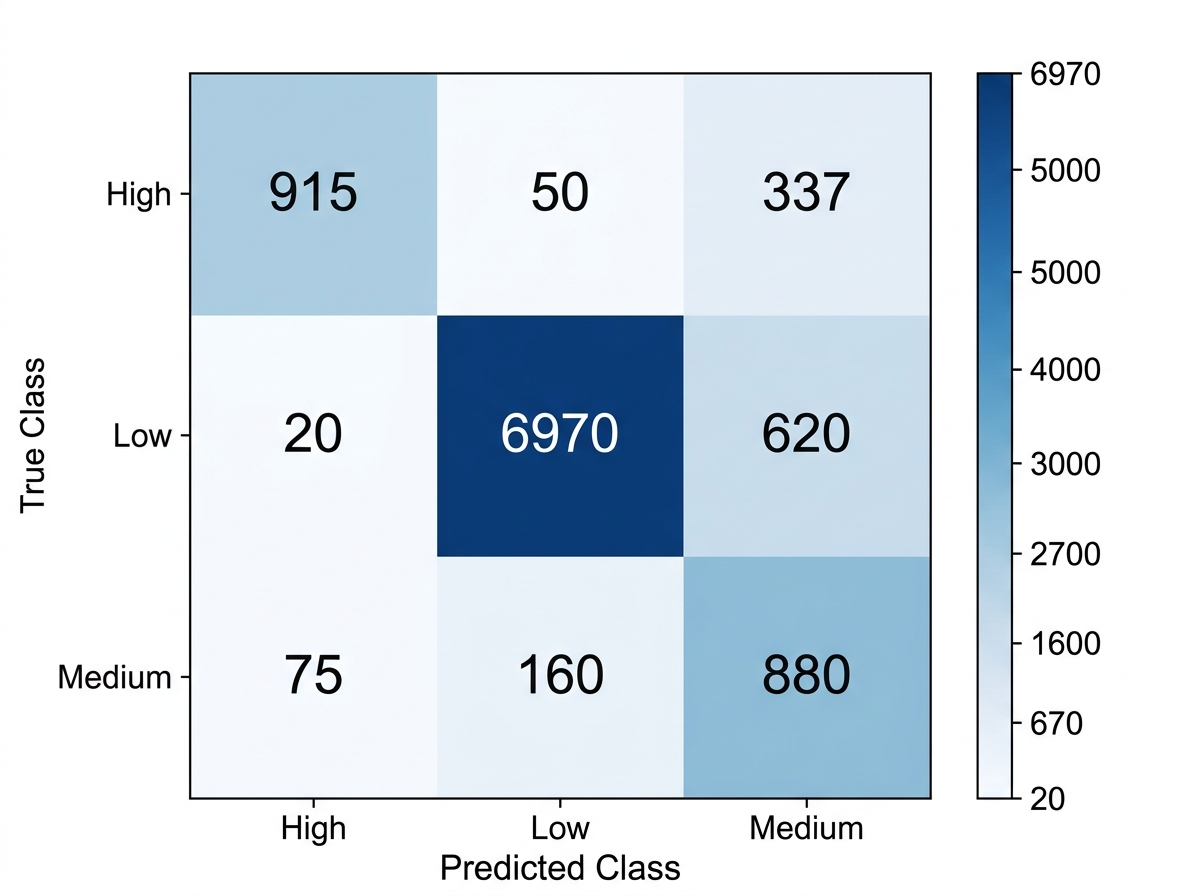
\includegraphics[width=0.88\linewidth]{figures/fig3_confusion_matrix.jpg}
\caption{Confusion Matrix for the Deployed Informer Model ($N = 10,027$).}
\label{fig:cm_informer}
\end{figure}

\subsection{Training Time Analysis}
Computational efficiency during training is essential for grid deployment scalability. Table \ref{tab:training_time} compares total execution time over 50 epochs across key deep learning architectures.

\begin{table}[htbp]
\caption{Training Time Comparison Across Key Architectures (50 Epochs)}
\centering
\resizebox{\columnwidth}{!}{%
\begin{tabular}{lc}
\toprule
\textbf{Model Architecture} & \textbf{Total Training Execution Time (Seconds)} \\
\midrule
\textbf{Informer (Primary)} & \textbf{111.20 s} \\
GRU & 149.85 s \\
LSTM & 168.27 s \\
TimesNet & 318.47 s \\
TFT & 332.51 s \\
PatchTST & 357.63 s \\
\bottomrule
\end{tabular}%
}
\label{tab:training_time}
\end{table}

Informer trained in 111.20 seconds, delivering a 3x speedup over TFT (332.51 s) and PatchTST (357.63 s) due to its ProbSparse attention mechanism.

\subsection{Statistical Validation}
To test whether accuracy differences among top models are statistically significant, we conducted paired McNemar's test ($\chi^2$) and Wilcoxon signed-rank tests across 10,027 test windows under significance threshold $\alpha = 0.05$.

Table \ref{tab:stat_tests} presents hypothesis test results. The null hypothesis ($H_0$: identical prediction performance) cannot be rejected for Informer vs. GRU ($p = 0.1166$), Informer vs. XGBoost ($p = 0.4756$), or Informer vs. Random Forest ($p = 0.8958$). Statistical significance ($p < 0.05$) was established only for Informer vs. TimesNet ($p = 0.0165$).

\begin{table}[htbp]
\caption{Pairwise Statistical Hypothesis Test Results ($\alpha = 0.05$)}
\centering
\resizebox{\columnwidth}{!}{%
\begin{tabular}{lcccc}
\toprule
\textbf{Comparison Pair} & \textbf{McNemar $\chi^2$} & \textbf{McNemar $p$} & \textbf{Wilcoxon $p$} & \textbf{Significance Status} \\
\midrule
Informer vs GRU & 2.463 & 0.1166 & 0.1036 & Not Significant ($p \ge 0.05$) \\
Informer vs XGBoost & 0.509 & 0.4756 & 0.4485 & Not Significant ($p \ge 0.05$) \\
Informer vs RF & 0.017 & 0.8958 & 0.8442 & Not Significant ($p \ge 0.05$) \\
Informer vs TimesNet & 5.752 & 0.0165 & 0.0138 & Significant ($p < 0.05$) \\
\bottomrule
\end{tabular}%
}
\label{tab:stat_tests}
\end{table}

\subsection{Controlled Feature Ablation}
To quantify the predictive impact of feature subsets, we conducted a controlled feature ablation study training five subset configurations under an accelerated retraining protocol (6 epochs, $lr = 0.002$, Full Model baseline = 88.42\% Accuracy, 77.78\% Macro F1).

As detailed in Table \ref{tab:ablation_results}, removing domain-engineered utilization indicators (\texttt{load\_utilization}, \texttt{demand\_utilization}, \texttt{renewable\_ratio}) produced the largest degradation (-1.56\% Macro F1 drop and -3.28\% Recall drop), confirming the value of domain feature engineering.

\begin{table}[htbp]
\caption{Controlled Ablation Study Performance Comparison}
\centering
\resizebox{\columnwidth}{!}{%
\begin{tabular}{lcccc}
\toprule
\textbf{Experiment Subset} & \textbf{Feat. Count} & \textbf{Accuracy} & \textbf{Macro F1} & \textbf{F1 Drop ($\Delta\%$)} \\
\midrule
Full Model (All Features) & 28 & 88.42\% & 77.78\% & Baseline (0.00\%) \\
-- Weather Variables & 21 & 88.40\% & 76.58\% & -1.53\% \\
-- Temporal Features & 24 & 88.32\% & 76.68\% & -1.41\% \\
-- Engineered Features & 21 & 88.36\% & 76.56\% & -1.56\% \\
Core Features Only & 14 & 88.15\% & 75.42\% & -3.03\% \\
\bottomrule
\end{tabular}%
}
\label{tab:ablation_results}
\end{table}

\subsection{Diurnal Robustness}
To evaluate model performance across daily operational shifts, we partitioned test predictions into four diurnal windows: Peak Hours (18:00--22:00), Off-Peak Hours, Daytime (06:00--17:00), and Nighttime (18:00--05:00).

Table \ref{tab:diurnal_results} shows that Informer exhibits stable performance across diurnal transitions, maintaining 87.29\% accuracy (71.71\% High-Risk recall) during Peak Hours and 87.45\% accuracy (69.84\% High-Risk recall) during Off-Peak Hours.

\begin{table}[htbp]
\caption{Diurnal Operational Performance Comparison}
\centering
\resizebox{\columnwidth}{!}{%
\begin{tabular}{lcccc}
\toprule
\textbf{Diurnal Condition} & \textbf{Model} & \textbf{Accuracy} & \textbf{Macro F1} & \textbf{High-Risk Recall} \\
\midrule
\multirow{3}{*}{Peak Hours (18--22h)} & Informer & 87.29\% & 77.73\% & 71.71\% \\
 & Random Forest & 87.21\% & 78.05\% & 71.38\% \\
 & XGBoost & 87.09\% & 76.27\% & 73.36\% \\
\midrule
\multirow{3}{*}{Off-Peak Hours} & Informer & 87.45\% & 77.65\% & 69.84\% \\
 & Random Forest & 87.44\% & 77.82\% & 69.24\% \\
 & XGBoost & 87.74\% & 76.22\% & 70.24\% \\
\bottomrule
\end{tabular}%
}
\label{tab:diurnal_results}
\end{table}

\subsection{Seasonal Robustness}
We evaluated model stability across three seasonal climatic regimes in Bangladesh: Summer (March--May), Monsoon (June--September), and Winter (November--February).

As presented in Table \ref{tab:seasonal_results} and Fig. \ref{fig:robustness_plots}, High-Risk recall drops across all models during the Summer partition (61.71\% for Informer) compared to Monsoon (91.30\%) and Winter (98.09\%), indicating that intense summer heatwave volatility creates complex load dynamics.

\begin{table}[htbp]
\caption{Seasonal Climatic Regime Performance Comparison}
\centering
\resizebox{\columnwidth}{!}{%
\begin{tabular}{lcccc}
\toprule
\textbf{Season} & \textbf{Model} & \textbf{Accuracy} & \textbf{Macro F1} & \textbf{High-Risk Recall} \\
\midrule
\multirow{3}{*}{Summer (Mar--May)} & Informer & 85.18\% & 76.53\% & 61.71\% \\
 & Random Forest & 84.84\% & 76.28\% & 61.19\% \\
 & XGBoost & 84.31\% & 74.07\% & 62.85\% \\
\midrule
\multirow{3}{*}{Monsoon (Jun--Sep)} & Informer & 91.11\% & 80.33\% & 91.30\% \\
 & Random Forest & 91.71\% & 81.78\% & 91.30\% \\
 & XGBoost & 91.71\% & 81.36\% & 91.30\% \\
\midrule
\multirow{3}{*}{Winter (Nov--Feb)} & Informer & 92.19\% & 72.66\% & 98.09\% \\
 & Random Forest & 92.69\% & 76.14\% & 96.82\% \\
 & XGBoost & 95.76\% & 75.62\% & 96.82\% \\
\bottomrule
\end{tabular}%
}
\label{tab:seasonal_results}
\end{table}

\begin{figure}[htbp]
\centering
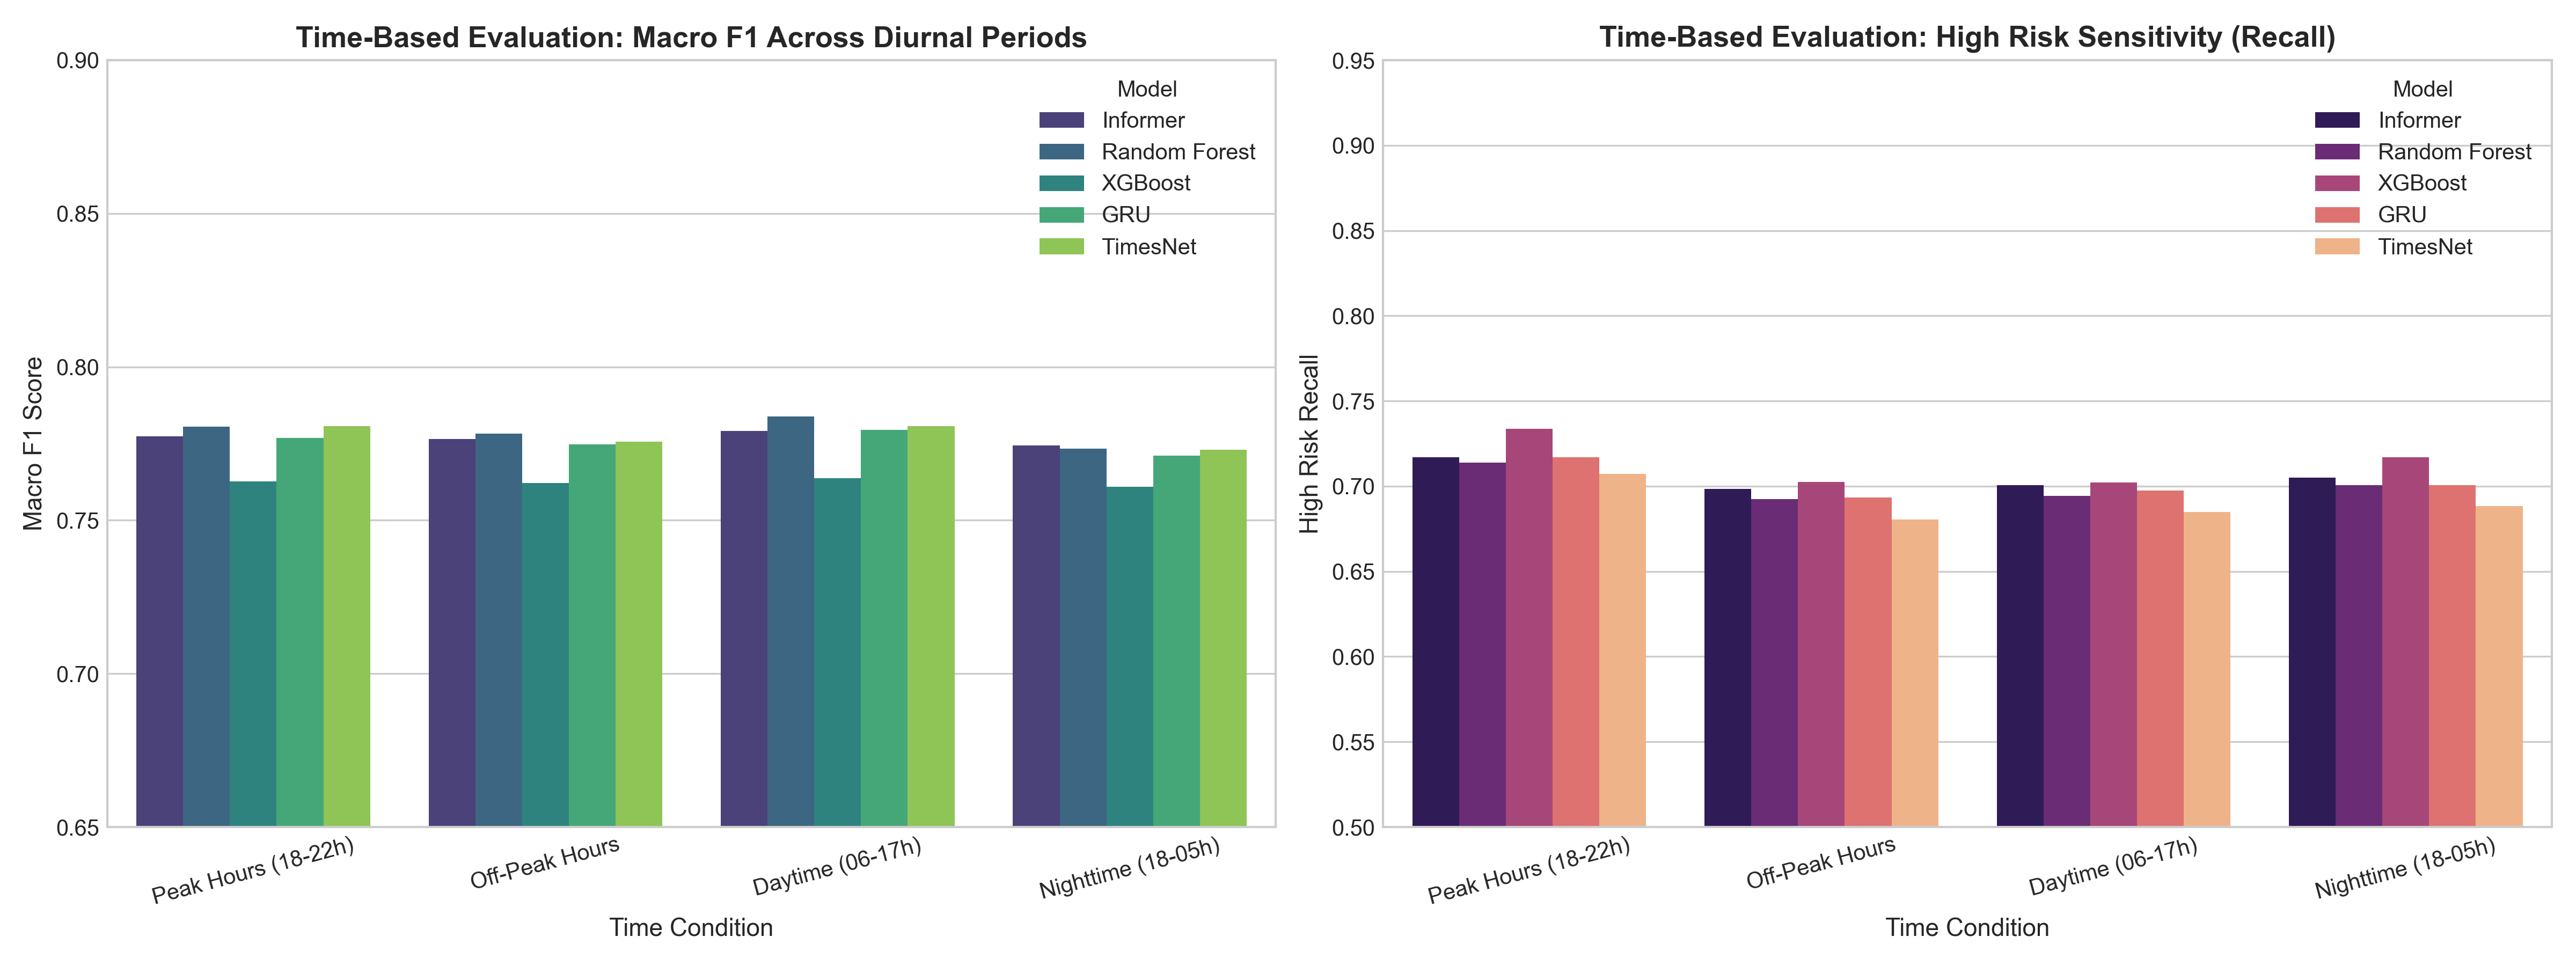
\includegraphics[width=0.88\linewidth]{figures/fig6_diurnal_seasonal_robustness.png}
\caption{Diurnal and Seasonal Robustness Evaluation Profiles.}
\label{fig:robustness_plots}
\end{figure}
